\PassOptionsToPackage{unicode=true}{hyperref} % options for packages loaded elsewhere
\PassOptionsToPackage{hyphens}{url}
\PassOptionsToPackage{dvipsnames,svgnames*,x11names*}{xcolor}
%
\documentclass[10pt,dvipsnames,enabledeprecatedfontcommands]{scrartcl}
\usepackage{lmodern}
\usepackage{amssymb,amsmath}
\usepackage{ifxetex,ifluatex}
\usepackage{fixltx2e} % provides \textsubscript
\ifnum 0\ifxetex 1\fi\ifluatex 1\fi=0 % if pdftex
  \usepackage[T1]{fontenc}
  \usepackage[utf8]{inputenc}
  \usepackage{textcomp} % provides euro and other symbols
\else % if luatex or xelatex
  \usepackage{unicode-math}
  \defaultfontfeatures{Ligatures=TeX,Scale=MatchLowercase}
\fi
% use upquote if available, for straight quotes in verbatim environments
\IfFileExists{upquote.sty}{\usepackage{upquote}}{}
% use microtype if available
\IfFileExists{microtype.sty}{%
\usepackage[]{microtype}
\UseMicrotypeSet[protrusion]{basicmath} % disable protrusion for tt fonts
}{}
\IfFileExists{parskip.sty}{%
\usepackage{parskip}
}{% else
\setlength{\parindent}{0pt}
\setlength{\parskip}{6pt plus 2pt minus 1pt}
}
\usepackage{xcolor}
\usepackage{hyperref}
\hypersetup{
            pdftitle={Boosting Legal Probabilism},
            pdfauthor={Marcello Di Bello and Rafal Urbaniak},
            colorlinks=true,
            linkcolor=Maroon,
            filecolor=Maroon,
            citecolor=Blue,
            urlcolor=blue,
            breaklinks=true}
\urlstyle{same}  % don't use monospace font for urls
\usepackage{graphicx,grffile}
\makeatletter
\def\maxwidth{\ifdim\Gin@nat@width>\linewidth\linewidth\else\Gin@nat@width\fi}
\def\maxheight{\ifdim\Gin@nat@height>\textheight\textheight\else\Gin@nat@height\fi}
\makeatother
% Scale images if necessary, so that they will not overflow the page
% margins by default, and it is still possible to overwrite the defaults
% using explicit options in \includegraphics[width, height, ...]{}
\setkeys{Gin}{width=\maxwidth,height=\maxheight,keepaspectratio}
\setlength{\emergencystretch}{3em}  % prevent overfull lines
\providecommand{\tightlist}{%
  \setlength{\itemsep}{0pt}\setlength{\parskip}{0pt}}
\setcounter{secnumdepth}{5}
% Redefines (sub)paragraphs to behave more like sections
\ifx\paragraph\undefined\else
\let\oldparagraph\paragraph
\renewcommand{\paragraph}[1]{\oldparagraph{#1}\mbox{}}
\fi
\ifx\subparagraph\undefined\else
\let\oldsubparagraph\subparagraph
\renewcommand{\subparagraph}[1]{\oldsubparagraph{#1}\mbox{}}
\fi

% set default figure placement to htbp
\makeatletter
\def\fps@figure{htbp}
\makeatother

%\documentclass{article}

% %packages
 \usepackage{booktabs}
 \usepackage[sort&compress]{natbib}
\usepackage{graphicx}
\usepackage{longtable}
\usepackage{ragged2e}
\usepackage{etex}
%\usepackage{yfonts}
\usepackage{marvosym}
\usepackage[notextcomp]{kpfonts}
\usepackage{nicefrac}
\newcommand*{\QED}{\hfill \footnotesize {\sc Q.e.d.}}
\usepackage{multicol} 
%\usepackage[textsize=footnotesize]{todonotes}
%\linespread{1.5}

\usepackage{xcolor}

\setlength{\parindent}{10pt}
\setlength{\parskip}{1pt}


%language
%\usepackage{times}
\usepackage{mathptmx}
\usepackage[scaled=0.88]{helvet}

\usepackage{t1enc}
%\usepackage[utf8x]{inputenc}
%\usepackage[polish]{babel}
%\usepackage{polski}

\usepackage{subcaption}


%AMS
\usepackage{amsfonts}
\usepackage{amssymb}
\usepackage{amsthm}
\usepackage{amsmath}

%\usepackage{geometry}
 %\geometry{a4paper,left=35mm,top=20mm,}

%abbreviations
\newcommand{\ra}{\rangle}
\newcommand{\la}{\langle}
\newcommand{\n}{\neg}
\newcommand{\et}{\wedge}
\newcommand{\jt}{\rightarrow}
\newcommand{\ko}[1]{\forall  #1\,}
\newcommand{\ro}{\leftrightarrow}
\newcommand{\exi}[1]{\exists\, {_{#1}}}
\newcommand{\pr}{\mathsf{P}}
\newcommand{\odds}{\mathsf{Odds}}
\newcommand{\ind}{\mathsf{Ind}}
\newcommand{\nf}[2]{\nicefrac{#1\,}{#2}}
\newcommand{\R}[1]{\texttt{#1}}

\newtheorem{q}{\color{blue}Question}


%% Rafal's stuff
\usepackage[margin=1.5in,top=1in]{geometry}
\usepackage[textsize=scriptsize, textwidth = 3cm]{todonotes}
% This is my own comment shading, keep \todo for general stuff, feel free to define your own separate comment colors (usually useful if you use margin comments at tall) For instance, I defined one for Patrycja
\newcommand{\rt}[1]{\todo[color = orange!40]{#1}}
\newcommand{\pt}[1]{\todo[color = blue!40]{#1}}




\newtheorem*{reply*}{Reply}
\usepackage{enumitem}
\newcommand{\question}[1]{\begin{enumerate}[resume,leftmargin=0cm,labelsep=0cm,align=left]
\item #1
\end{enumerate}}

\usepackage{float}

% \setbeamertemplate{blocks}[rounded][shadow=true]
% \setbeamertemplate{itemize items}[ball]
% \AtBeginPart{}
% \AtBeginSection{}
% \AtBeginSubsection{}
% \AtBeginSubsubsection{}
% \setlength{\emergencystretch}{0em}
% \setlength{\parskip}{0pt}

\title{Boosting Legal Probabilism}
\author{Marcello Di Bello and Rafal Urbaniak}
\date{}

\begin{document}
\maketitle

\hypertarget{the-book}{%
\section{The Book}\label{the-book}}

\hypertarget{brief-description}{%
\subsection{Brief Description}\label{brief-description}}

\footnotesize In one or two paragraphs, describe the work, including its
rationale, approach, and pedagogy. (This book is\ldots{} It does\ldots{}
Its distinguishing features are\ldots{})

\normalsize

Can the evidence presented at trial be examined, weighed and assessed
using probability theory? Can legal decision-making and standards of
proof such as `preponderance of the evidence' or `proof beyond a
reasonable doubt' be defined using the language of probability and
expected utility? Does the deployment of probability theory in assessing
evidence and making decisions improve the accuracy and fairness of legal
decision-making? Over the last fifty years, these questions have been
extensively debated in the literature in philosophy, law, forensic
science and artificial intelligence. Legal probabilism is a research
program whose supporters believe that the answer to these questions is,
by and large, affirmative. Others, however, hold a less optimistic view.
`Boosting Legal Probabilism' examines the most important objections to
this research program and articulates a version of legal probabilism
that is able to address many, if not all, of these objections.

We first articulate the simple version of legal probabilism. This
version has much to be reccomeded for, but also falls prey to several
difficulties, including the problem of conjunction, puzzles of naked
statistical evidence, the problem of priors. Some legal probabilists
have attempted to dismiss these difficulties or downplay their
significance. We confront them at face value and show they cannot be
addressed within the confines of simple legal probabilism. We then
develop a more sophisticated version of the theory, what we call legal
probabilism 1.02, which deploys Bayesian networks and takes advantage of
seminal ideas in the literature in forensic science and artificial
intelligence. `Boosting Legal Probabilism' articulates the first
comprehensive philosophical analysis of whether---and if so, to what
extent---legal probabilism 1.02 can overcome the limitations of simple
legal probabilism. We show that the more sophisticated version
significantly improves on the simple version and rivals in explanatory
power two competing accounts of judicial fact-finding: argumentation
theory and relative plausibility. To add precision to the claims made in
the book, the analytical argument is supplemented with an
\textbf{\textsf{R}} code implementation.

`Boosting Legal Probabilism' is aimed at philosophers with an interest
in legal epistemology and epistemology more generally. Many of the
difficulties of legal probabilism resemble difficulties faced by
Bayesianism in epistemology. The book will also draw attention outside
philosophy from legal scholars who have championed applications of
probability theory to evidence law as well as scholars who have resisted
this trend. Another target audience includes computer scientists and
psychologists interested in studying evidential reasoning and
decision-making under uncertainty. Besides contributing to the
literature about legal probabilism, the book aims to introduce
unfamiliar readers to the rich interdisciplinary debate on the topic,
often scattered throughout journals and books in philosophy, law,
computer science, forensic science and psychology. So the book is aimed
at scholars, advanced undergraduates and curios readers more generally.
Some chapters present original research and require technical background
in probability theory. Others are introductory, suitable for an advanced
undergraduate course.

\hypertarget{outline}{%
\subsection{Outline}\label{outline}}

\noindent \textbf{Part I}

\noindent The first part of the book outlines simple legal probabilism
(Chapter 1) and its foes (Chapter 2). The simple version comprises a
familiar repertoire: Bayes' theorem, likelihood ratios, probability
thresholds, expected utility maximization. This repertoire has proven
useful in several ways, especially in the assessment of explicitly
quantitative evidence such as DNA matches and other expert evidence. At
the same time, simple legal probabilism is liable to a host of
conceptual difficulties: the conjunction problem, the problem of priors,
paradoxes of naked statistical evidence. These difficulties are
well-known. Others are less familiar: the problem of complexity, soft
variables, the difficulty with corroboration.

Part I is meant to instill interest in the topic among unfamiliar
readers and refresh seasoned readers about the main points of
contention. Part I provides the essential background for a deeper
examination of legal probabilism and the development of its more
sophisticated version. The remaining two parts of the book covers two
separate topics: evidence assessment (Part II) and decision-making (Part
III). This distinction reflects the fact that legal probabilism is both
a theory of evidence assessment (or evidence evaluation, evidence
weighing) as well as a theory of decision-making at trial. These two
topics are obviously intertwined in important ways, but are best kept
separate for analytical clarity.

\vspace{3mm}

\noindent \textbf{Part II}

\noindent The second part of the book discusses in great detail three
formal tools used for the assessment of evidence from a probabilistic
perspective: Bayes' theorem, likelihood ratios and Bayesian networks.
This part discusses how these formal tools can help to assess, weigh and
evaluate evidence at trial as well as what their limitations are. The
objective of this part of the book is to articulate a more sophisticated
version of legal probabilism for evidence assessment which overcomes the
difficulties of the simpler version.

Chapter 3 begins with Bayes' theorem and illustrates how the theorem can
be put to use in weighing pieces of evidence at trial. Bayes' theorem is
useful in many ways, for example, to avoid reasoning fallacies such as
the prosecutor's fallacy and the base rate fallacy. At the same time,
its applications are also limited. As discussed in Chapter 4, court
cases often require fact-finders to weigh several pieces of evidence,
sometimes conficting and susceptible to different interpretations. The
hypotheses that the fact-finders are asked to evaluate in light of the
evidence are structured stories or explanations constituted by several
sub-propositions. This level of complexity can hardly be modeled by a
simple application of Bayes' theorem. A more sophisticated machinery for
evidence assessment is nedded.

Before discussing this more sophisticated machinery, the book describes
a formal tool that is, in some important way, an alternative to Bayes'
theorem and that many legal probabilists have found useful: likelihood
ratios. Bayes' theorem requires one to assess the prior probabilities of
the hypothesis of interest. The problem is that assessing prior
probabilities is notoriously difficult. Likelihood ratios offer a way to
evaluate the evidence presented at trial without the need of assessing
prior probabilities. Chapter 5 illustrates the many applications of
likelihood ratios focusing on the debate about cold-hit DNA matches as
an illustration. The chapter also examines the weaknesses of the
likelihood ratio approach, in particular, the chapter details how the
choice of the competing hypotheses to be compared in the likelihood
ratio is often a source of confusion, manipulation and subjective
judgment. A further problem is that, like Bayes' theorem, likelihood
ratios are still unable to model complex bodies of evidence.

Chapters 3, 4 and 5 -- combined -- show that we need to move past simple
legal probabilism. The journey toward legal probabilism 1.02 is
accomplished in Chapters 6 through 10. We focus on two aspects of the
evaluation of trial evidence which simple legal probabilism is unable to
model: first, judges and jurors often think holistically about the
evidence, say in terms of coherent stories or explanations, without
assessing the evidence by discrete applications of Bayes' theorem or
likelihood ratios; second, different pieces of evidence interact in
complex relationships, such as undercutting, rebutting, converging,
corroborating evidence. We show that Bayesian networks constitute the
formal machinery for developing a more sophisticated legal probabilism
that is able to formally capture these phenomena.

Chapter 6 offers a crash course on Bayesian networks with a focus on the
assessment of legal evidence. A Bayesian network comprises a directed
acyclic graph (called a DAG) that represents relations of dependence
between variables, along with conditional probability tables
corresponding to these relations. Simple graphical patterns called
`idioms' often appear while modeling the relationships between evidence
and hypotheses. In the last decade, the literature in artificial
intelligence and forensic science has made significant progress in
modeling holistic notions such as the coherence of a story and
argument-based notions such as conflicts between pieces of evidence.
Chapter 6 surveys this literature focusing on the work of Charlotte Vlek
and Norman Fenton. Vlek, together with Bart Verheij and Henry Prakken,
proposed to model the coherence of a story by adding a node in the
Bayesian network, call it a `story node'. The story node has other nodes
as its children. These correspond to the events that make up the story.
In turn, these events are linked to their supporting evidence. An
example of a Bayesian network with a story node (or scenario node to use
Vlek's terminology) is depicted below:

\begin{center}
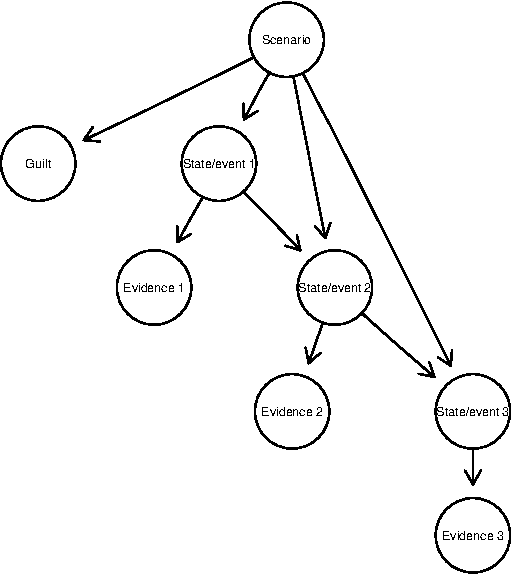
\includegraphics[width=8cm]{vlek-scenario-node.pdf}
 \end{center}

Since the story node unifies the different parts of a story, changes in
the probabilities of these parts can be used to model the notion of
coherence. The stronger the (positive) probabilistic dependency between
the different parts, the more coherent the story. There may also be
competing stories about what happened, say, one story was put forward by
the prosecution and another by the defense. A Bayesian network can be
built that comprises two competing stories and specifies that they are
incompatible and cannot be true concurrently. Another approach to model
competing stories was developed by Norman Fenton and his research group.
Separate stories are represented by separate Bayesian networks, and
Bayesian model comparison is then used for assessing the relative
strenght of the competing stories.

Chapter 7 and 8 articulate different lines of criticism of Vlek's and
Fenton's formalizations. The criticisms are followed by our positive
proposal that still relies, like Vlek's and Fenton's, on Bayesian
networks. Chapter 7 focuses on weakenessses of the story node approach
as an account of coherence. We show that adding a story node by fiat --
without any good reason for supposing that the different parts of the
story are connected other than being part of one story -- introduces
unnecessary probabilistic dependencies between the elements of a story.
Since these dependencies may or may not exist, they should be assessed
on a case-by-case basis and modeled accordingly. In addition, the story
node approach is overly simplistic as an account of coherence and fails
to engage with the rich philosophical literature on the topic. After the
critical part, Chapter 7 articulates a more adequate probabilistic
account of the coherence of a story. Instead of adding a story node, we
show that it is more appropriate to assess the dependency between the
different parts of a story on a case-by-case basis and build the
Bayesian network accordingly. {[}THIS FEELS A BIT THIN. ANYTHING ELSE
HERE TO DESCRIBE THE POSITIVE ACCOUNT OF COHERENCE? ANYTHING TO ADD?{]}

Chapter 8 and 9 focus on complex relantionships between pieces of
evidence, such as conflicting evidence and corroborating evidence. A
criticism we level against Vlek's story node approch and Fenton's model
comparison approach is that they both fail to capture crucial aspects of
how pieces of evidence and competing stories conflict with one another
at trial. It is too simplistic to posit that the complex adversarial
dialectic that takes place in a trial could be modeled by averaging
different Bayesian networks (Fenton) or postulating relationships of
incompatibility between different story nodes (Vlek). We need an account
of more fine-grained notions, such as undercutting and rebutting
evidence, and more generally we need an accounf of how cross-examimation
operates at trial. What cross-examination often accomplishes is not so
much the creation of an alternative story, but rather the
reinterpretation of an existign story by supplying additional
information As chapter 8 illustrates, this process of reintepretation
can be represented formally as the refinement of an existing Bayesian
network. We show that, by drawing additional arrows between evidence
nodes and hypothesis nodes, conflicts between pieces of evidence such as
undercutting and rebutting can be modeled adequately.

The reverse of the phenomenon of conflicting evidence is that of
converging evidence, in particular, the fact that one piece of evidence
corroborates another. Corroboration has been the focus of extensive
scholarly debate often outside the literature in legal probabilism.
Chapter 9 surveys the probabilistic literature on corroboration and the
main difficulties that have been levelled against the proposed accounts.
The chapter then formalizes a notion of corroboration based on Bayesian
networks that overcomes most of the difficulties of the exisisting
accounts. {[}ANYTHING ELSE HERE TO DESCRIBE THE POSITIVE ACCOUNT OF
CORROBORATION?{]}

Chapter 10 summarizes our proposal for legal probabilism 1.02, limited
to the realm of evidence asessment at trial, draws some general morals
and compares our proposal to competing accounts. In preceeding chapters,
we show that legal probabilism 1.02 -- roughly, simple legal probabilism
supplemented by Bayesian networks -- can represent complex relationships
between pieces of evidence such as undercutting and corroboration
(Chapters 8 and 9), as well as holistic notions such as coherence
(Chapter 7). The key idea is that the coherence of a story as well as
conflicts between pieces of evidence can be modeled formally in terms of
corresponding properties of, operations on, and relations between
Bayesian networks. Our formal analysis was guided by the followign
working hypothesis: An accusation of liability must be substantiated by
providing a well-specified account -- story, narrative -- of the alleged
illegal act committed by the defendant. This account consists of several
moving parts, each supported by different items of evidence. The defense
may respond by attacking the supporting evidence, the internal
consistency of the account, or by offerring an alternative account.
Judges and jurors are tasked with assessing how well the claim that the
defendant is civilly or criminally liable is supported by the evidence
and how well it stands up against criticism. It is this complex dynamics
that we attemped to formalize in the preceeding chapters.

Chapter 10 compares our proposed version of legal probabilism 1.02 with
two competing accounts of judicial fact-finding: argumentation theory
and relative plausibility. We suggest that our theory outperforms these
comepting accounts in some respect, although we do not claim that it
outperforme them on all counts. First, argumentation theory does not
offer a clear account of degrees of evidential strenght. Evidence may
supports a hypothesis more or less strongly, or two pieces of evodence
may conflcts with one another more less strongly. Not only does legal
probabilism 1.02 offer an account of evidenetila support, coinflict and
convergence, but the account is nuanced enough to capture degrees of
support, conflict and converegence. This is marked improvement. Second,
relative plausibility is often critized because the defense need not
always present a full-fledged alternative story or alternative
explaination of the evidence. The critisism is that it should be enough
for the defense to challenge the story or explanation proposed by the
party, say the prosecution in a criminal case. We do not take a stance
on this controversy, but we note that legal probabilism 1.02 is flexible
enough to model competing stories or explanations (in agreement with
relative plausibility) and alternatively model conflicts between pieces
of evidence without the need to construct a full-fledged alternative
story or explanation (as critics of relative plausibility prefer). There
remains, however, a fundamental difficulty with legal probabilism 1.02,
its cognitive plausibility. It is not clear that the process of evidence
assessment naturally conforms to the probabilistic machinery. In fact,
it most likely does not. This difficulty does not undermine legal
probabilism 1.02 as a theory of evidence assessment, but it certainly
quesions its emprical adequacy as a theory of evidence assessment at
trial. In this respect, relative plausibility -- and perhpas
argumentation theory -- fares much better.

MAYBE ADD OUR ACCOUNT CAN CAPTURE THINGS LIKE COMPLETENESS OF EVIDEMCE,
SPECIFICITY OF A NARRATIVE, WHETHER A PIECE OF EVIDENCE IS INDEPENDENTLY
SECURED, CROSSWORD PUZZLE ANALOGY AND SUSAN HAACK.

\vspace{3mm}

\noindent \textbf{Part III}

The final part of the book examines trial-decision making, specifically,
to what extent standards of proof such as `preponderance of the
evidence' and `proof beyond a reasonable doubt' can be understood
through the lenses of probability theory.

\vspace{3mm}

\noindent \textbf{Table of contents}

\renewcommand{\labelenumi}{\Roman{enumi}}
\renewcommand{\labelenumii}{\arabic{enumii}}
\renewcommand{\labelenumiii}{\arabic{enumii}.\arabic{enumiii}}

\begin{enumerate}
\item Legal probabilism 1.01 and its foes
\begin{enumerate}

  \item The emergence of legal probabilism
  \begin{enumerate}
  \item  Famous cases
  \item  Probabilistic evidence
  \item  Trial by mathematics
  \item  Some history
  \end{enumerate}
  

  
  \item  A skeptical perspective
  \begin{enumerate}
  \item  The difficulty about conjunction
  \item  The problem of priors
  \item  Naked statistical evidence
  \item  The complexity problem
  \item  Soft variables
  \item  Corroboration
  \item  The reference class problem
  \item  Non-probabilistic theories
  \end{enumerate}


\end{enumerate}
\item  Evidence assessment


\begin{enumerate}


\setcounter{enumii}{2}
  \item  Bayes' Theorem and the usual fallacies
  \begin{enumerate}
  \item  Assuming independence
  \item  The prosecutor's fallacy
  \item  Base rate fallacy
  \item  Defense attorney's fallacy
  \item  Uniqueness fallacy
  \item  Case studies
  \end{enumerate}

  
  
  \item  Complications and caveats
  \begin{enumerate}
  \item  Complex hypotheses and complex bodies of evidence
  \item Source, activity and offense level hypotheses
  \item  Where do the numbers come from?
  \item  Modeling corroboration
  \item  Stories, explanations and coherence
  \end{enumerate}

  
  \item  Likelihood Ratios and Relevance
  \begin{enumerate}
  \item Likelihood ratio as a measure of evidence strength
  \item The risk of false positive and its impact
  \item Hypothesis choice
  \item Levels of hypotheses and the two-stain problem
  \item Relevance and the small-town murder scenario
  \item The cold-hit confusion
  \item  Likelihood ratio and  cold-hit DNA matches
  \end{enumerate}



  \item  Bayesian Networks
  \begin{enumerate}
  \item  Bayesian networks to the rescue
  \item  Legal evidence idioms
  \item Scenario idioms
  \item Modeling relevance
  \item  Case study: Sally Clark
  \item DNA evidence
  \end{enumerate}
  
  \item Conflicts
  \begin{enumerate}
  \item Argumenation theory
  \item Undercutting and rebutting evidence
  \item Cross-examination
  \item Conflicting evidence in Bayesian networks
  \end{enumerate}
 
 
  \item Corroboration
  \begin{enumerate}
  \item Boole's formula and Cohen's challenge
  \item  Modeling substantial rise in case of agreement
  \item Ekel\"of's corroboration measure and evidentiary mechanisms
  \item General approach with multiple false stories and multiple witnesses
  \end{enumerate}


  \item Coherence
  \begin{enumerate}
  \item  Existing probabilistic coherence measures
  \item  An array of counterexamples
  \item Coherence of structured narrations with Bayesian networks
  \item  Application to legal cases
  \end{enumerate}

  \item  New legal probabilism
    \begin{enumerate}
    \item  Desiderata
    \item  A probabilistic framework for narrations
    \item  Probabilistic explications of the desiderata
    \item  Bayesian network implementation
    \end{enumerate}


\end{enumerate}
\item  Trial Decisions
\begin{enumerate}



\setcounter{enumii}{10}
  \item  The functions of the proof standards
  \begin{enumerate}
  \item  Conceptual desiderata
  \item  Protecting defendants
  \item  Error reduction and error distribution/allocation
  \item  Dispute resolution and public deference
  \item  Justification and answerability
  \end{enumerate}



  \item  Standards of proof
  \begin{enumerate}
  \item  Legal background
  \item  Probabilistic thresholds
  \item  Theoretical challenges
  \item  Specific narratives
  \item The comparative strategy
  \item  The likelihood strategy
  \item Challenges (again)
  \item Probabilistic thresholds revised
  \item  Bayesian networks and probabilistic standard of proof
  \end{enumerate}

  \item  Accuracy and the risk of error
  \begin{enumerate}
  \item  Minimizing expected costs
  \item  Minimizing expected errors
  \item  Expected v.\ actual errors
  \item  Competing accounts of the risk of error
  \item  Bayesian networks and the risk of error
  \end{enumerate}



  \item  Fairness in trial decisions
  \begin{enumerate}
  \item  Procedural v.\ substantive fairness
  \item  Competing measures of substantive fairness
  \item  Bayesian networks and fairnesss
  \end{enumerate}


  \item  Alternative accounts and legal probabilism
  \begin{enumerate}
  \item  Baconian probability
  \item  Relative Plausibility
  \item  Arguments
  \item  Sensitivity
  \item  Normic Support
  \item  Justification/foundherentism
  \item  Completeness
  \item  Relevant alternatives
  \item  Knowledge
  \end{enumerate}

\item Conclusions
\end{enumerate}
\end{enumerate}

\hypertarget{outstanding-features-of-the-book}{%
\subsection{Outstanding Features of the
Book}\label{outstanding-features-of-the-book}}

\begin{itemize}
\item
  (First) comprehensive sustained philosophical discussion of legal
  probabilism.
\item
  Multi-faceted in its incorporation of insights from various
  discussions present in legal, philosophical, and forensic research.
\item
  With a practical accent, due to the implementation of the conceptual
  points by means of bayesian networks and \textbf{\textsf{R}}
  programming language.
\end{itemize}

\todo{what else?}

\hypertarget{apparatus}{%
\subsection{Apparatus}\label{apparatus}}

\footnotesize a. Will the book include photographs, line drawings,
cases, questions, problems, glossaries, bibliography, references,
appendices, etc.?

\vspace{2mm}

\normalsize

Yes, the book will contain various plots, either of Bayesian networks,
or some other data visualisations generated by \texttt{ggplot2}. The
book also will contain bibliography. \vspace{2mm}

\footnotesize b. If the book is a text, do you plan to provide
supplementary material to accompany it? (Teacher's manual, study guide,
solutions, answers, workbook, anthology, or other material.)

\vspace{2mm}

\normalsize

The book will be accompanied by an online-only appendix detailing the
use of the \texttt{R} code in the book and the source code we used.

\hypertarget{competition}{%
\subsection{Competition}\label{competition}}

\footnotesize a. Consider the existing books in this field and discuss
specifically their strengths and weaknesses. Spell out how your book
will be similar to, as well as different from, competing works.

\todo{For now, let's list competition, and discuss key differences}

\normalsize

Three types: BNs in the law, Philosophy \& law, Statistics in law and
forensics

\begin{itemize}
\item
  ``Bayesian Networks and Probabilistic Inference in Forensic Science''
  by Taroni, Aitken, Garbolino and Biedermann.
\item
  ``Risk Assessment and Decision Analysis with Bayesian Networks'' by
  Fenton and Neil.
\item
  ``Bayesian Networks With Examples in R'' by Marco Scutari and
  Jean-Baptiste Denis.
\item
  Alex Stein, foundations of evidence law
\item
  Nance, Burdens of proof
\item
  Schauer, Profiles, \dots
\item
  Ho, Philosophy of evidence law
\item
  Robertson, Vignaux
\item
  Lucy Dawid,
\item
  Statistics for Lawyers etc.
\end{itemize}

\begin{enumerate}
\def\labelenumi{\alph{enumi}.}
\setcounter{enumi}{1}
\item
  Consider what aspects of topical coverage are similar to or different
  from the competition. What topics have been left out of competing
  books and what topics have been left out of yours?
\item
  Please discuss each competing book in a separate paragraph. (If
  possible, please provide us with the publisher and date of publication
  as well.) This information will provide the reviewers and the
  publisher a frame of reference for evaluating your material. Remember,
  you are writing for reviewers and not for publication, so be as frank
  as possible regarding your competition. Give credit where credit is
  due, and show how you can do it better.
\end{enumerate}

\hypertarget{market-considerations}{%
\section{Market Considerations}\label{market-considerations}}

\hypertarget{the-primary-market}{%
\subsection{The Primary Market}\label{the-primary-market}}

\begin{enumerate}
\def\labelenumi{\arabic{enumi}.}
\item
  What is the major market for the book? (Scholarly/professional, text,
  reference, trade?)
\item
  If this is a text, for what course is the book intended? Is the book a
  core text or a supplement? What type of student takes this course?
  What is the level? (Major or non-major; freshman, senior, graduate?)
  Do you offer this course yourself? If so, how many times have you
  given it? Is your text class-tested?
\item
  If the market is scholarly/professional, reference, or trade, how may
  it best be reached? (Direct mail, relevant journals, professional
  associations, libraries, book or music stores?) For what type of
  reader is your book intended?
\end{enumerate}

\hypertarget{status-of-the-work}{%
\section{Status of the Work}\label{status-of-the-work}}

\begin{enumerate}
\def\labelenumi{\arabic{enumi}.}
\tightlist
\item
  Do you have a timetable for completing the book?
\end{enumerate}

\begin{enumerate}
\def\labelenumi{\alph{enumi}.}
\item
  What portion or percentage of the material is now complete?
\item
  When do you expect to have a complete manuscript?
\end{enumerate}

\begin{enumerate}
\def\labelenumi{\arabic{enumi}.}
\setcounter{enumi}{1}
\tightlist
\item
  What do you estimate to be the size of the completed book?
\end{enumerate}

\begin{enumerate}
\def\labelenumi{\alph{enumi}.}
\item
  Double spaced typewritten pages normally reduce about one-third when
  set in type; e.g., 300 typewritten pages make about 200 printed pages.
  There are about 450 words on a printed page.
\item
  Approximately how many photographs do you plan to include?
\item
  Approximately how many line drawings (charts, graphs, diagrams, etc. )
  will you need?
\item
  Do you plan to include material requiring permission (text, music,
  lyrics, illustrations)? To what extent? Have you started the
  permissions request process?
\end{enumerate}

\begin{enumerate}
\def\labelenumi{\arabic{enumi}.}
\setcounter{enumi}{2}
\tightlist
\item
  Do you plan to class-test the material in your own or other sections
  of the course? (Any material distributed to students should be
  protected by copyright notice on the material.)
\end{enumerate}

\hypertarget{sample-chapters}{%
\section{Sample Chapters}\label{sample-chapters}}

Select one or two chapters of the manuscript that are an integral part
of the book. They should be those you consider the best-written ones,
and do not have to be in sequence. For example, you might submit
chapters 3, 7, and 14 of a 20-chapter book, so long as these chapters
represent the content and reflect your writing style and pedagogy in the
best possible light. It is also advisable to submit any chapter that is
particularly innovative or unique. Sample chapters should contain rough
sketches, charts, hand-written musical examples or xerox reproductions,
and description of photographs to be included. The material need not be
in final form, although it should be carefully prepared and represent
your best work. In your preparation, emphasis should be on readability.
Please do not bind your manuscript, as we will have to unbind it in
order to make photocopies for reviewers. Also be sure all pages are
numbered either consecutively or double-numbered by chapter.

\hypertarget{reviews}{%
\section{Reviews}\label{reviews}}

If we are interested in your project, we will commission outside
reviewers to read and evaluate your proposal. We will, of course, obtain
the best available reviewers to consider your work. If you wish to
suggest the names of experts in your field whom you believe to be
ideally suited to evaluate your proposal, you may provide their names,
titles, and email addresses. While we are unlikely to approach these
scholars to act as reviewers themselves, we may ask them for their
suggestions for peer readers. Naturally, we do not reveal the names of
reviewers without their permission.

\hypertarget{author-background}{%
\section{Author Background}\label{author-background}}

Please include a current CV or brief biography of your writing,
teaching, and/or educational background and experience. Be sure to list
any books that you have previously published, and any other information
about yourself on why you are qualified to write this book.

\hypertarget{response-time}{%
\section{Response Time}\label{response-time}}

Please allow at least 6-10 weeks for the manuscript proposal evaluation
and review process. We will contact you as soon as we have had a chance
to thoroughly examine your manuscript proposal. Thank you for your
interest in Oxford University Press. We look forward to reading your
materials.

\end{document}
